\documentclass[aspectratio=169,sn-mathphys-num]{beamer}

\usepackage{fontspec}
\usepackage{unicode-math}
\usepackage{graphicx}
\usepackage[dvipsnames]{xcolor}
\usepackage[sorting=none]{biblatex}
\usepackage{ragged2e}
\usepackage{setspace}
\usepackage{bookmark}
\usepackage{mhchem}
\usepackage[spanish]{babel}

\addbibresource{../references.bib}

\usetheme[numbering=counter, progressbar=frametitle, background=light]{metropolis}

\usecolortheme{dove}
\definecolor{primary}{RGB}{88, 24, 124}
\definecolor{secondary}{RGB}{0, 168, 150}

\setbeamercovered{transparent}
\setbeamercolor{frametitle}{fg=white, bg=primary}
\setbeamercolor{progress bar}{fg=secondary}
\setbeamerfont{frametitle}{size=\large, series=\bfseries}
\setbeamerfont{title}{size=\LARGE, series=\bfseries}
\setbeamercolor{alerted text}{fg=secondary}
\setbeamercolor{block title}{fg=primary}
\setbeamercolor{block body}{bg=white}

\setstretch{1.1}

\setmainfont{Fira Sans}
\setmathfont{TeX Gyre Pagella Math}

\title{Cerámicos: Alfarería y Superconductores}
\subtitle{La física, evolución y aplicación}
\author{Avila, Herrera, Acuña, Martinez}
\institute{Universidad Distrital Francisco José de Caldas}
\date{\today}

\begin{document}

\begin{frame}
	\titlepage
\end{frame}

\begin{frame}{Outline}
	\setbeamertemplate{section in toc}[sections numbered]
	\tableofcontents
\end{frame}

\section{Propiedades Físicas}

\begin{frame}{Definiendo los Cerámicos: Más que Alfarería}
	\begin{block}{Definición Central}
		Sólidos inorgánicos, no metálicos, típicamente preparados mediante
		calentamiento y posterior enfriamiento.
	\end{block}

	\begin{itemize}
		\item Esta simple definición oculta una vasta complejidad en su química,
			estructura y propiedades.
		\item La clave para entender los cerámicos reside en sus enlaces
			interatómicos.
	\end{itemize}
\end{frame}

\begin{frame}{El Corazón de los Cerámicos: Enlaces Interatómicos}
	\begin{columns}[T]
		\begin{column}{0.5\textwidth}
			\begin{alertblock}{Enlaces Cerámicos Primarios}
				Caracterizados por fuertes \textbf{enlaces iónicos y/o covalentes}.
				\begin{itemize}
					\item Alta energía de enlace.
					\item Fuerzas intensas, a menudo direccionales.
				\end{itemize}
			\end{alertblock}
		\end{column}
		\begin{column}{0.5\textwidth}
			\begin{exampleblock}{En Contraste}
				\begin{itemize}
					\item \textbf{Metálico}: Mar de electrones, no direccional.
					\item \textbf{Polimérico}: Fuerzas débiles de van der Waals.
				\end{itemize}
			\end{exampleblock}
		\end{column}
	\end{columns}

	\begin{block}{Consecuencias del Enlace Fuerte}
		Altos puntos de fusión, dureza significativa y excelente estabilidad química.
	\end{block}
\end{frame}

\begin{frame}{Estructura Cristalina: Orden vs. Caos}
	\begin{columns}[T] % El entorno de columnas ya está creado

		% --- Columna Izquierda: Cristalino ---
		\begin{column}{0.5\textwidth}
			\begin{block}{Cristalinos (Ordenados)}
				Estructura atómica repetitiva y de largo alcance.

				% --- Comando para insertar la imagen ---
				\begin{figure}
					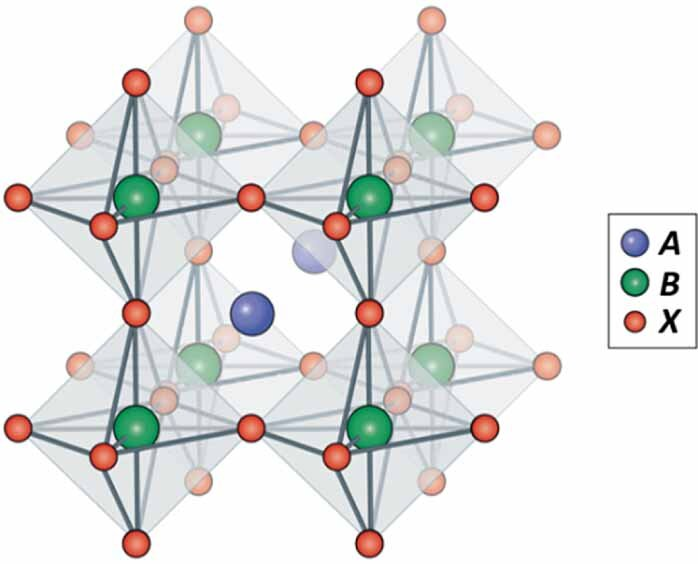
\includegraphics[width=0.7\linewidth]{../figures/perovskite-crystal-structure-CaTiO3-ABX3.jpg}
					\caption{Ej: Estructura de Perovskita (\ce{CaTiO3}) \cite{ng_group-iii-nitride_2021}}
				\end{figure}

			\end{block}
		\end{column}

		% --- Columna Derecha: Amorfo ---
		\begin{column}{0.5\textwidth}
			\begin{block}{Amorfos (Desordenados)}
				Estructura atómica sin un orden a largo plazo.

				% --- Comando para insertar la imagen ---
				\begin{figure}
					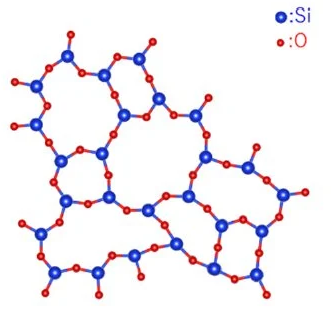
\includegraphics[width=0.6\linewidth]{../figures/Schematic-of-silica-molecule.png}
					\caption{Ej: Red de sílice vítrea (\ce{SiO2}) \cite{kohara_relationship_2011}}
				\end{figure}

			\end{block}
		\end{column}

	\end{columns}
\end{frame}

\begin{frame}{Estructura-Propiedad I: Comportamiento Mecánico}
	\begin{alertblock}{El Problema de la Fragilidad}
		Alta resistencia a la compresión, pero baja resistencia a la tracción y
		tenacidad a la fractura ($K_{IC}$).
	\end{alertblock}

	\begin{itemize}
		\item \textbf{Teoría de la Fractura Frágil de Griffith}: Defectos
			nanoscópicos preexistentes (\textit{grietas de Griffith}) actúan como
			concentradores de esfuerzo, llevando a una falla catastrófica bajo
			tensión.
			\pause
		\item \textbf{Razón Fundamental}: Los enlaces fuertes y direccionales
			resisten el movimiento de dislocaciones. La energía se libera mediante la
			propagación de grietas, no por deformación plástica.
	\end{itemize}
\end{frame}

\begin{frame}{Estructura-Propiedad II: Propiedades Térmicas y Eléctricas}
	\begin{columns}[T]
		\begin{column}{0.5\textwidth}
			\begin{block}{Propiedades Térmicas}
				\begin{itemize}
					\item Generalmente baja conductividad térmica debido a la
						\textbf{dispersión de fonones} efectiva en redes cristalinas
						complejas.
					\item Alta estabilidad térmica debido a la alta energía de enlace.
				\end{itemize}
			\end{block}
		\end{column}
		\begin{column}{0.5\textwidth}
			\begin{block}{Propiedades Eléctricas}
				\begin{itemize}
					\item Excelentes aislantes. Explicado por la \textbf{teoría de
						bandas}: una gran banda prohibida ($E_g$) previene la excitación de
						electrones.
					\item Los defectos/dopaje pueden crear estados en la banda prohibida,
						conduciendo a un comportamiento semiconductor.
				\end{itemize}
			\end{block}
		\end{column}
	\end{columns}
\end{frame}

\begin{frame}{Clasificación: Una Historia de Dos Cerámicos}
	\begin{block}{Cerámicos Tradicionales}
		\begin{itemize}
			\item Productos a base de arcilla (alfarería, ladrillo, porcelana).
			\item Compuestos de materias primas naturales no refinadas.
		\end{itemize}
	\end{block}
	\vspace{1cm}
	\begin{alertblock}{Cerámicos Avanzados / Técnicos}
		\begin{itemize}
			\item Materiales sintéticos de alta pureza diseñados para un rendimiento
				funcional o estructural específico.
			\item Ejemplos: \ce{Al2O3}, \ce{Si3N4}, \ce{BaTiO3}.
		\end{itemize}
	\end{alertblock}
\end{frame}


\begin{frame}{El Desafío de las Altas Temperaturas}
  \frametitle{Requerimientos Térmicos en la Nueva Siderurgia}
  El desarrollo industrial impuso condiciones operativas que excedían la
  capacidad de los materiales convencionales.

  \begin{columns}[T]
    \begin{column}{0.6\textwidth}
      \begin{itemize}[<+->]
        \item La producción de \textbf{acero} a escala industrial y la
          optimización de \textbf{máquinas de vapor} requerían hornos y calderas
          que operaran a temperaturas sostenidas y elevadas.
        \item Los materiales de construcción existentes, como ladrillos comunes
          y mampostería, sufrían fallas estructurales y fusión bajo estas
          condiciones.
      \end{itemize}
    \end{column}
    \begin{column}{0.4\textwidth}
      \begin{figure}
        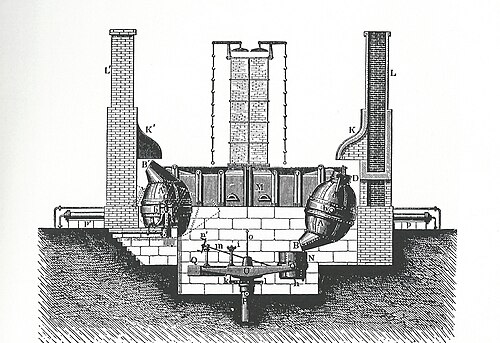
\includegraphics[width=\textwidth]{../figures/bessemer.jpg}
        \caption{Convertidor Bessemer. \cite{wiki:bessemer}}
      \end{figure}
    \end{column}
  \end{columns}
\end{frame}

\begin{frame}{Aplicación de Cerámicos Refractarios}
  \frametitle{Soluciones para la Contención Térmica}
  La solución técnica se basó en el desarrollo de cerámicos especializados.

  \begin{columns}[T]
    \begin{column}{0.6\textwidth}
      \begin{itemize}[<+->]
        \item Se industrializó la producción de ladrillos a partir de
          \textbf{arcillas refractarias (fireclay)} y \textbf{sílice
          (\ce{SiO2})}.
        \item Su función principal fue el revestimiento interno de altos hornos,
          convertidores y calderas.
        \item \textbf{Impacto técnico:} La capacidad de contener energía térmica
          fue un requisito indispensable para la siderurgia moderna.
      \end{itemize}
    \end{column}
    \begin{column}{0.4\textwidth}
      \begin{figure}
        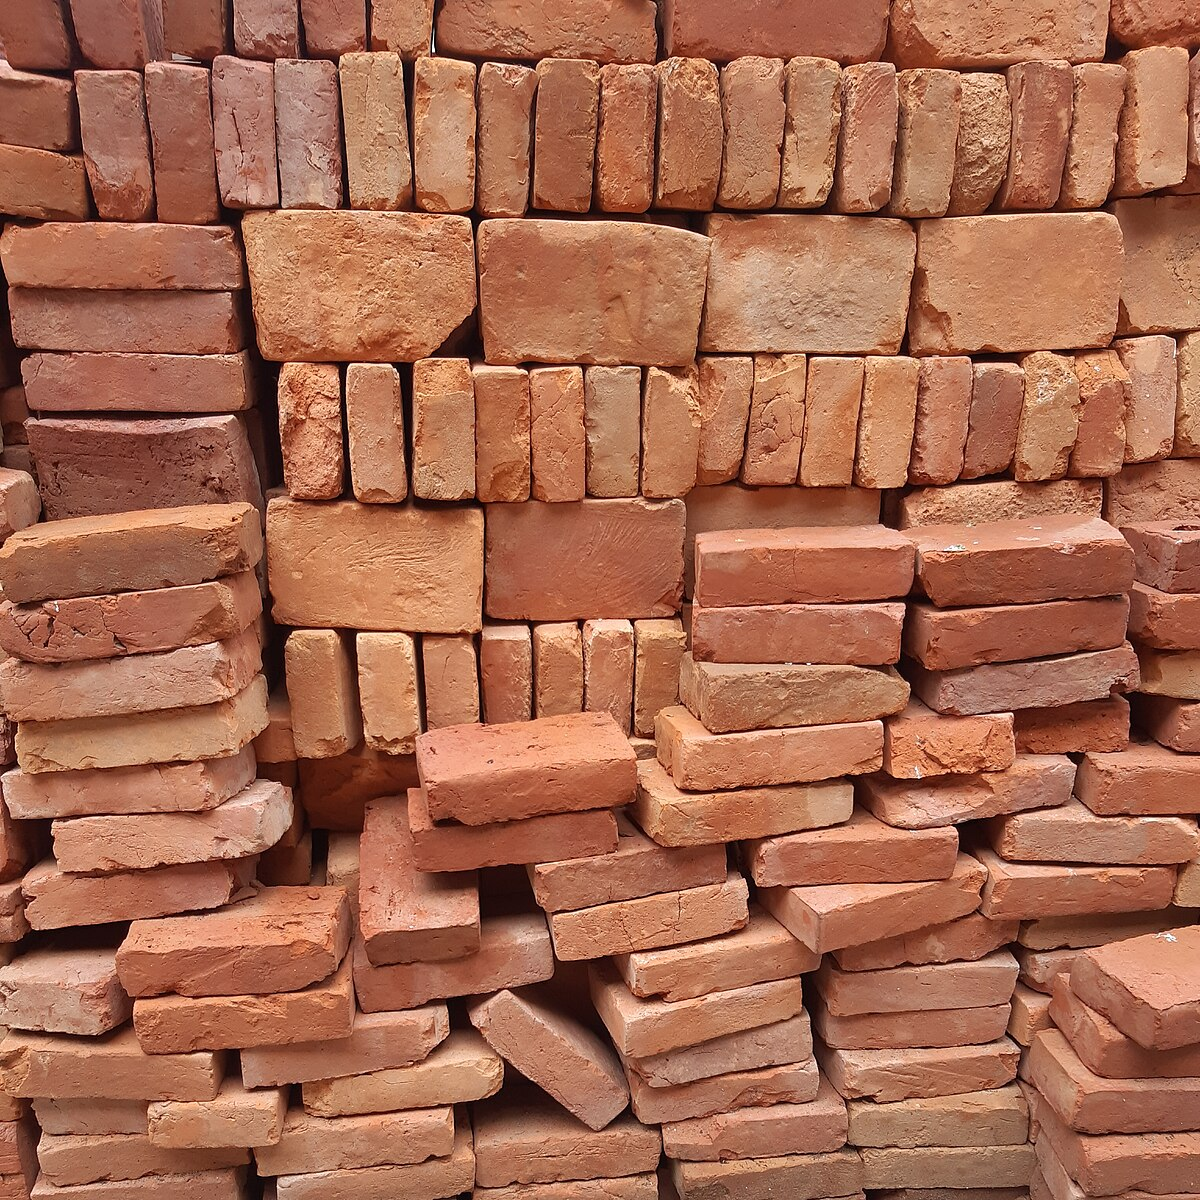
\includegraphics[width=\textwidth]{../figures/refractory_bricks.jpg}
        \caption{Bloques de Ladrillos. \cite{wiki:fired_bricks}}
      \end{figure}
    \end{column}
  \end{columns}
\end{frame}

\begin{frame}{Contención de Agentes Corrosivos}
  La emergente industria química requería recipientes y ductos con alta inercia
  química.

  \begin{columns}[T]
    \begin{column}{0.6\textwidth}
      \begin{itemize}[<+->]
        \item El \textbf{gres cerámico vitrificado} se estableció como el
          material estándar por su baja porosidad y alta resistencia a ácidos.
        \item Se empleó en la fabricación de contenedores y tuberías para la
          producción de ácido sulfúrico.
      \end{itemize}
    \end{column}
    \begin{column}{0.4\textwidth}
      \begin{figure}
        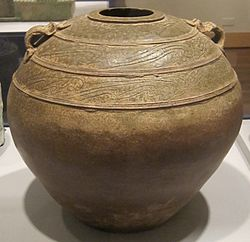
\includegraphics[width=0.8\textwidth]{../figures/stoneware_jars.jpg}
        \caption{Alfarería de Piedra. \cite{wiki:stoneware}}
      \end{figure}
    \end{column}
  \end{columns}
\end{frame}

\begin{frame}{Rol en la Infraestructura Sanitaria}
  \frametitle{Materiales para el Saneamiento Urbano}
  La rápida urbanización demandó soluciones duraderas para la gestión de aguas
  residuales.

  \begin{columns}[T]
    \begin{column}{0.6\textwidth}
      \begin{itemize}[<+->]
        \item La crisis sanitaria en centros industriales impulsó el desarrollo
          de redes de saneamiento a gran escala.
        \item Las \textbf{tuberías de gres vitrificado} ofrecían la durabilidad
          e impermeabilidad necesarias para los primeros sistemas de
          alcantarillado.
      \end{itemize}
    \end{column}
    \begin{column}{0.4\textwidth}
      \begin{figure}
        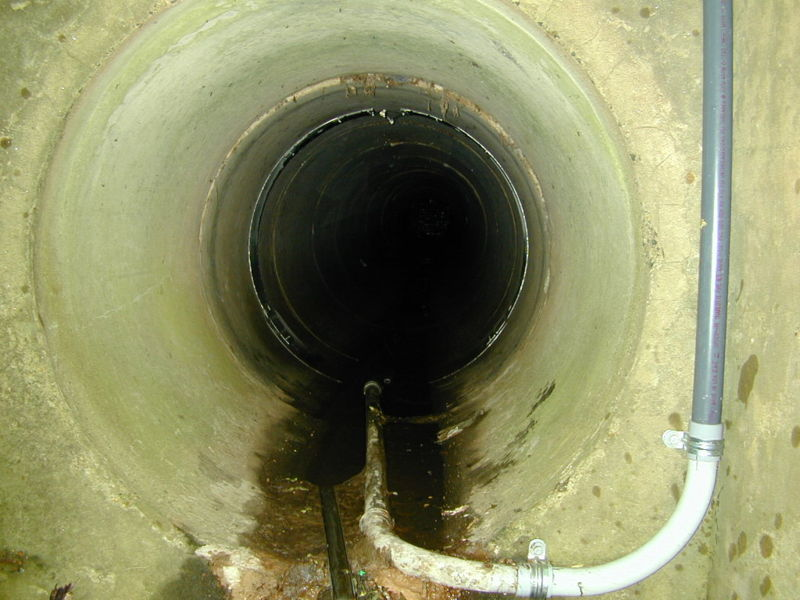
\includegraphics[width=\textwidth]{../figures/sewer_pipes.jpg}
        \caption{Alcantarillas. \cite{wiki:sewer}}
      \end{figure}
    \end{column}
  \end{columns}
\end{frame}

\begin{frame}{El Problema del Aislamiento Eléctrico}
  \frametitle{Requerimientos para la Transmisión de Energía}
  La distribución de energía eléctrica presentaba un desafío fundamental: su
  aislamiento seguro y eficiente.

  \begin{columns}[T]
    \begin{column}{0.6\textwidth}
      \begin{itemize}[<+->]
        \item Se necesitaba un material de \textbf{alta resistividad
          dieléctrica} para prevenir pérdidas de corriente y cortocircuitos.
        \item Dicho material debía poseer \textbf{estabilidad mecánica y
          ambiental} para su uso en exteriores.
      \end{itemize}
    \end{column}
    \begin{column}{0.4\textwidth}
      \begin{figure}
        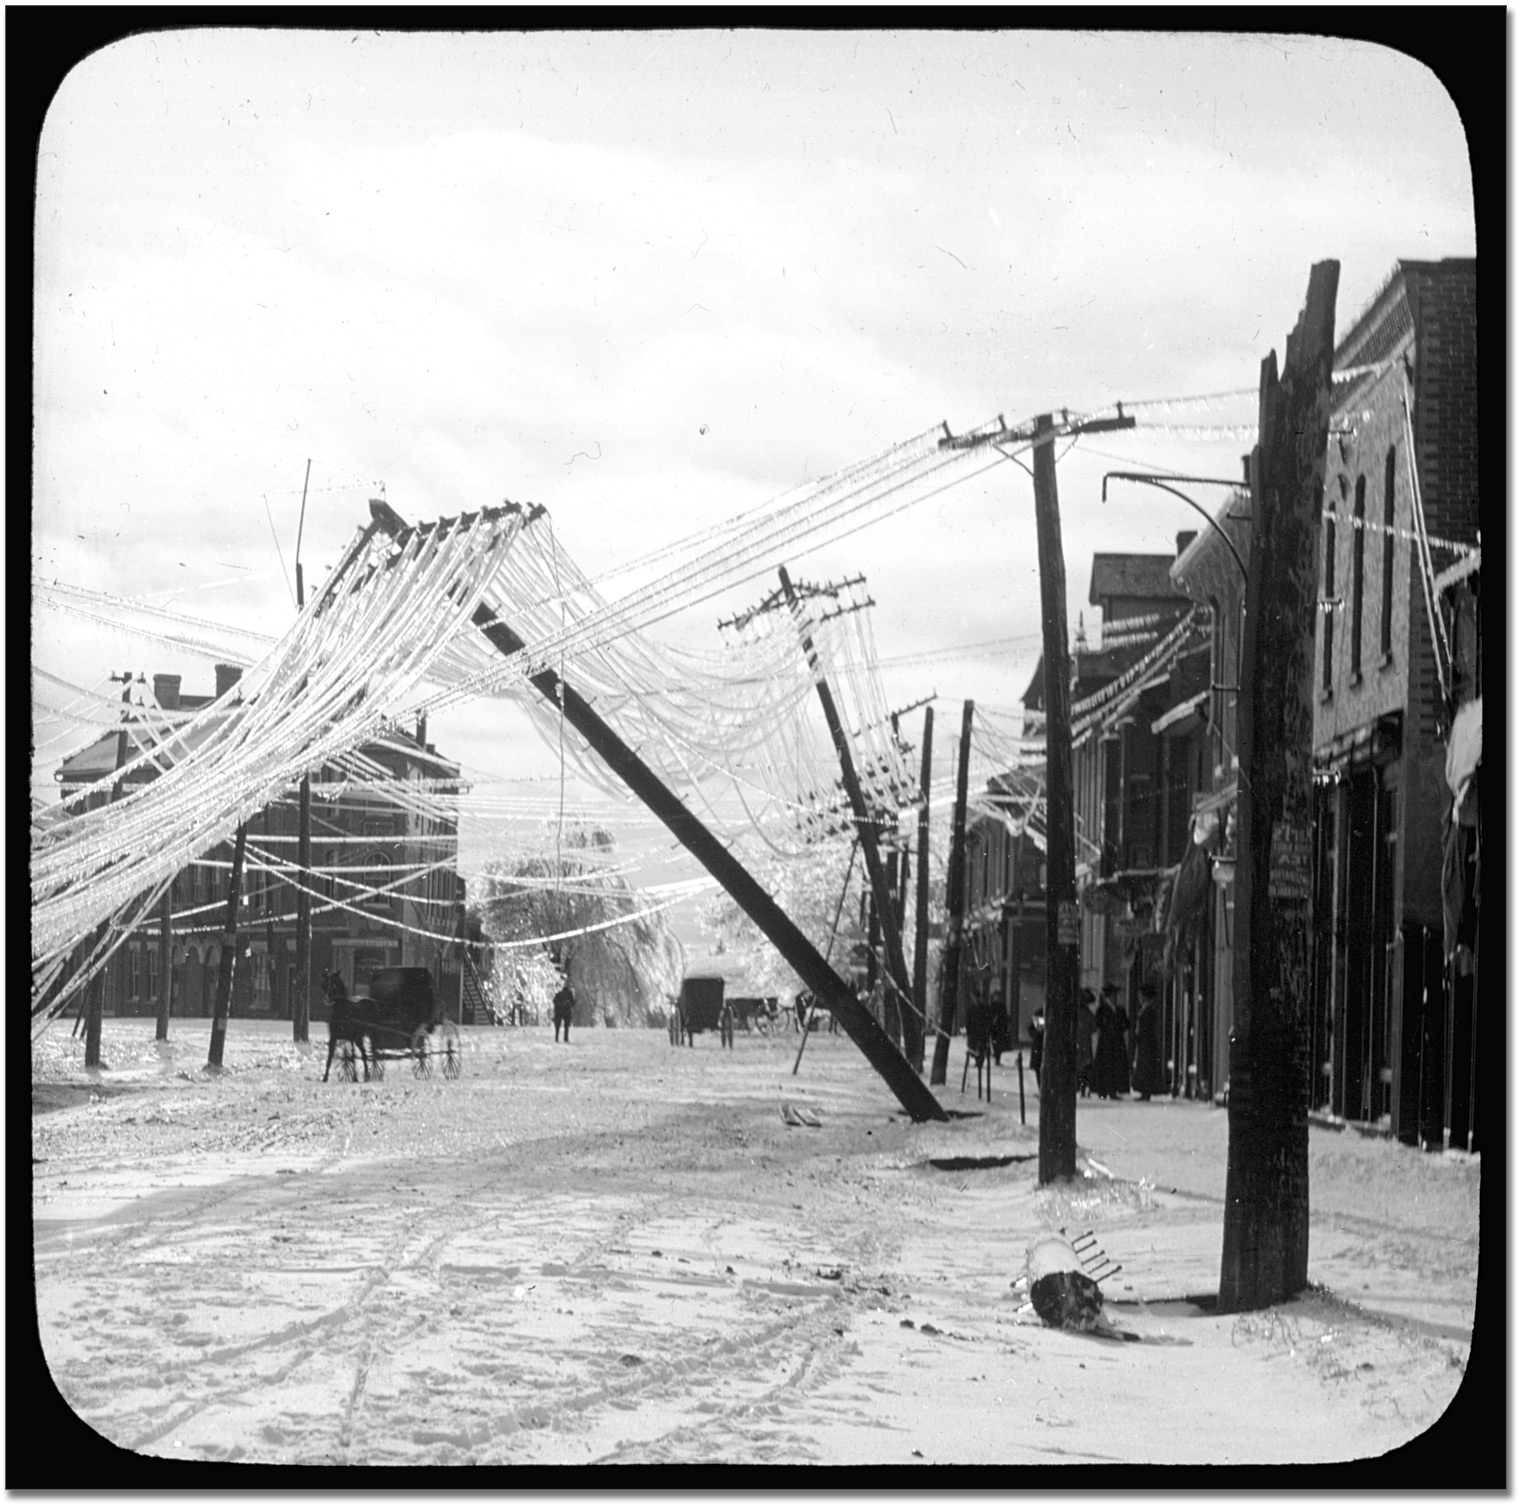
\includegraphics[width=0.8\textwidth]{../figures/early_power_lines.jpg}
        \caption{Tormenta en Ontario. \cite{wiki:ice_storm_photo}}
      \end{figure}
    \end{column}
  \end{columns}
\end{frame}

\begin{frame}{La Porcelana como Aislante Eléctrico}
  \frametitle{Material Dieléctrico Estándar}
  La cerámica, una vez más, proveyó la solución técnica óptima.

  \begin{columns}[T]
    \begin{column}{0.6\textwidth}
      \begin{itemize}[<+->]
        \item La \textbf{porcelana eléctrica}, densa a base de caolín,
          feldespato y cuarzo, demostró tener propiedades dieléctricas y
          mecánicas superiores.
        \item Su principal aplicación fue la fabricación en masa de
          \textbf{aisladores} para las redes de telegrafía, telefonía y
          transmisión de energía.
      \end{itemize}
    \end{column}
    \begin{column}{0.4\textwidth}
      \begin{figure}
        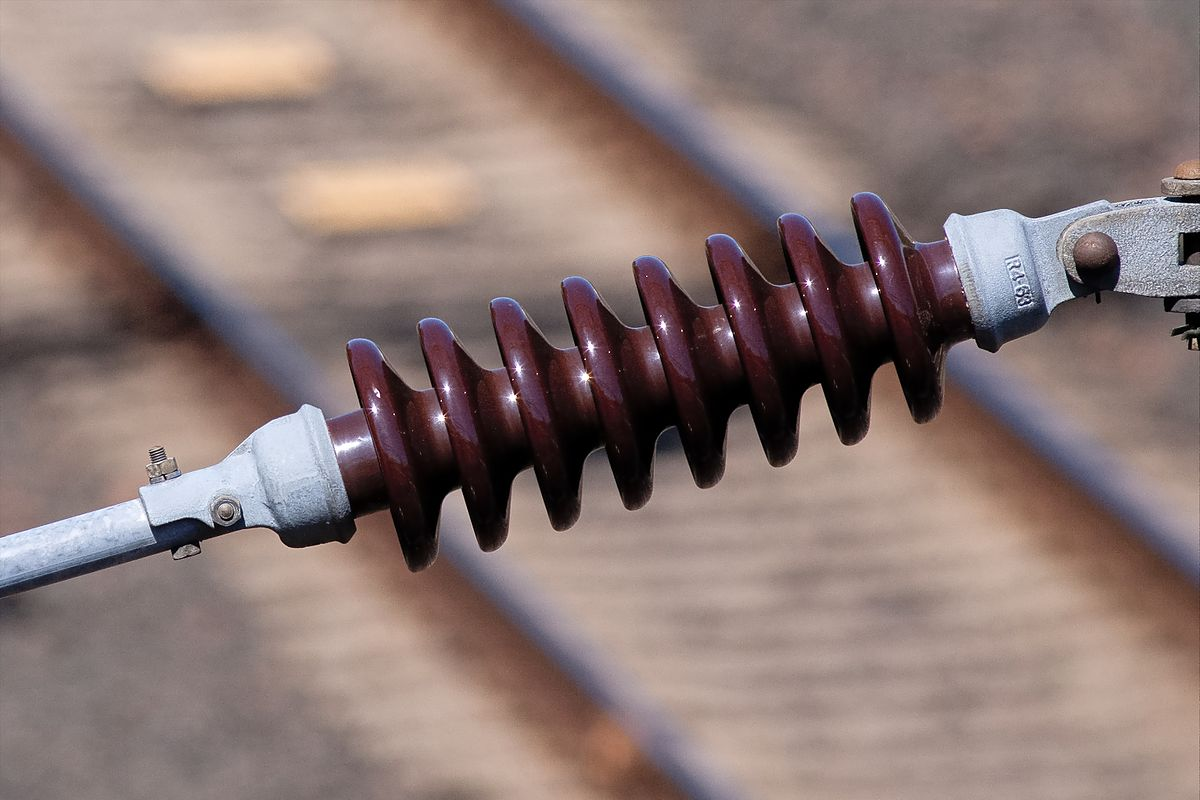
\includegraphics[width=\textwidth]{../figures/porcelain_insulators.jpg}
        \caption{Aislantes cerámicos. \cite{wiki:insulator}}
      \end{figure}
    \end{column}
  \end{columns}
\end{frame}

\begin{frame}{Nuevos Requerimientos para la Electrónica}
  \frametitle{El Advenimiento de los Circuitos Eléctricos}
  El desarrollo de la radio y la telegrafía sin hilos introdujo nuevos
  requerimientos a nivel de componente.

  \begin{columns}[T]
    \begin{column}{0.6\textwidth}
      \begin{itemize}[<+->]
        \item Los componentes electrónicos requerían materiales que ofrecieran
          \textbf{aislamiento eléctrico a pequeña escala}.
        \item Adicionalmente, era necesaria una alta \textbf{estabilidad
          dimensional y térmica} para garantizar el funcionamiento fiable.
      \end{itemize}
    \end{column}
    \begin{column}{0.4\textwidth}
      \begin{figure}
        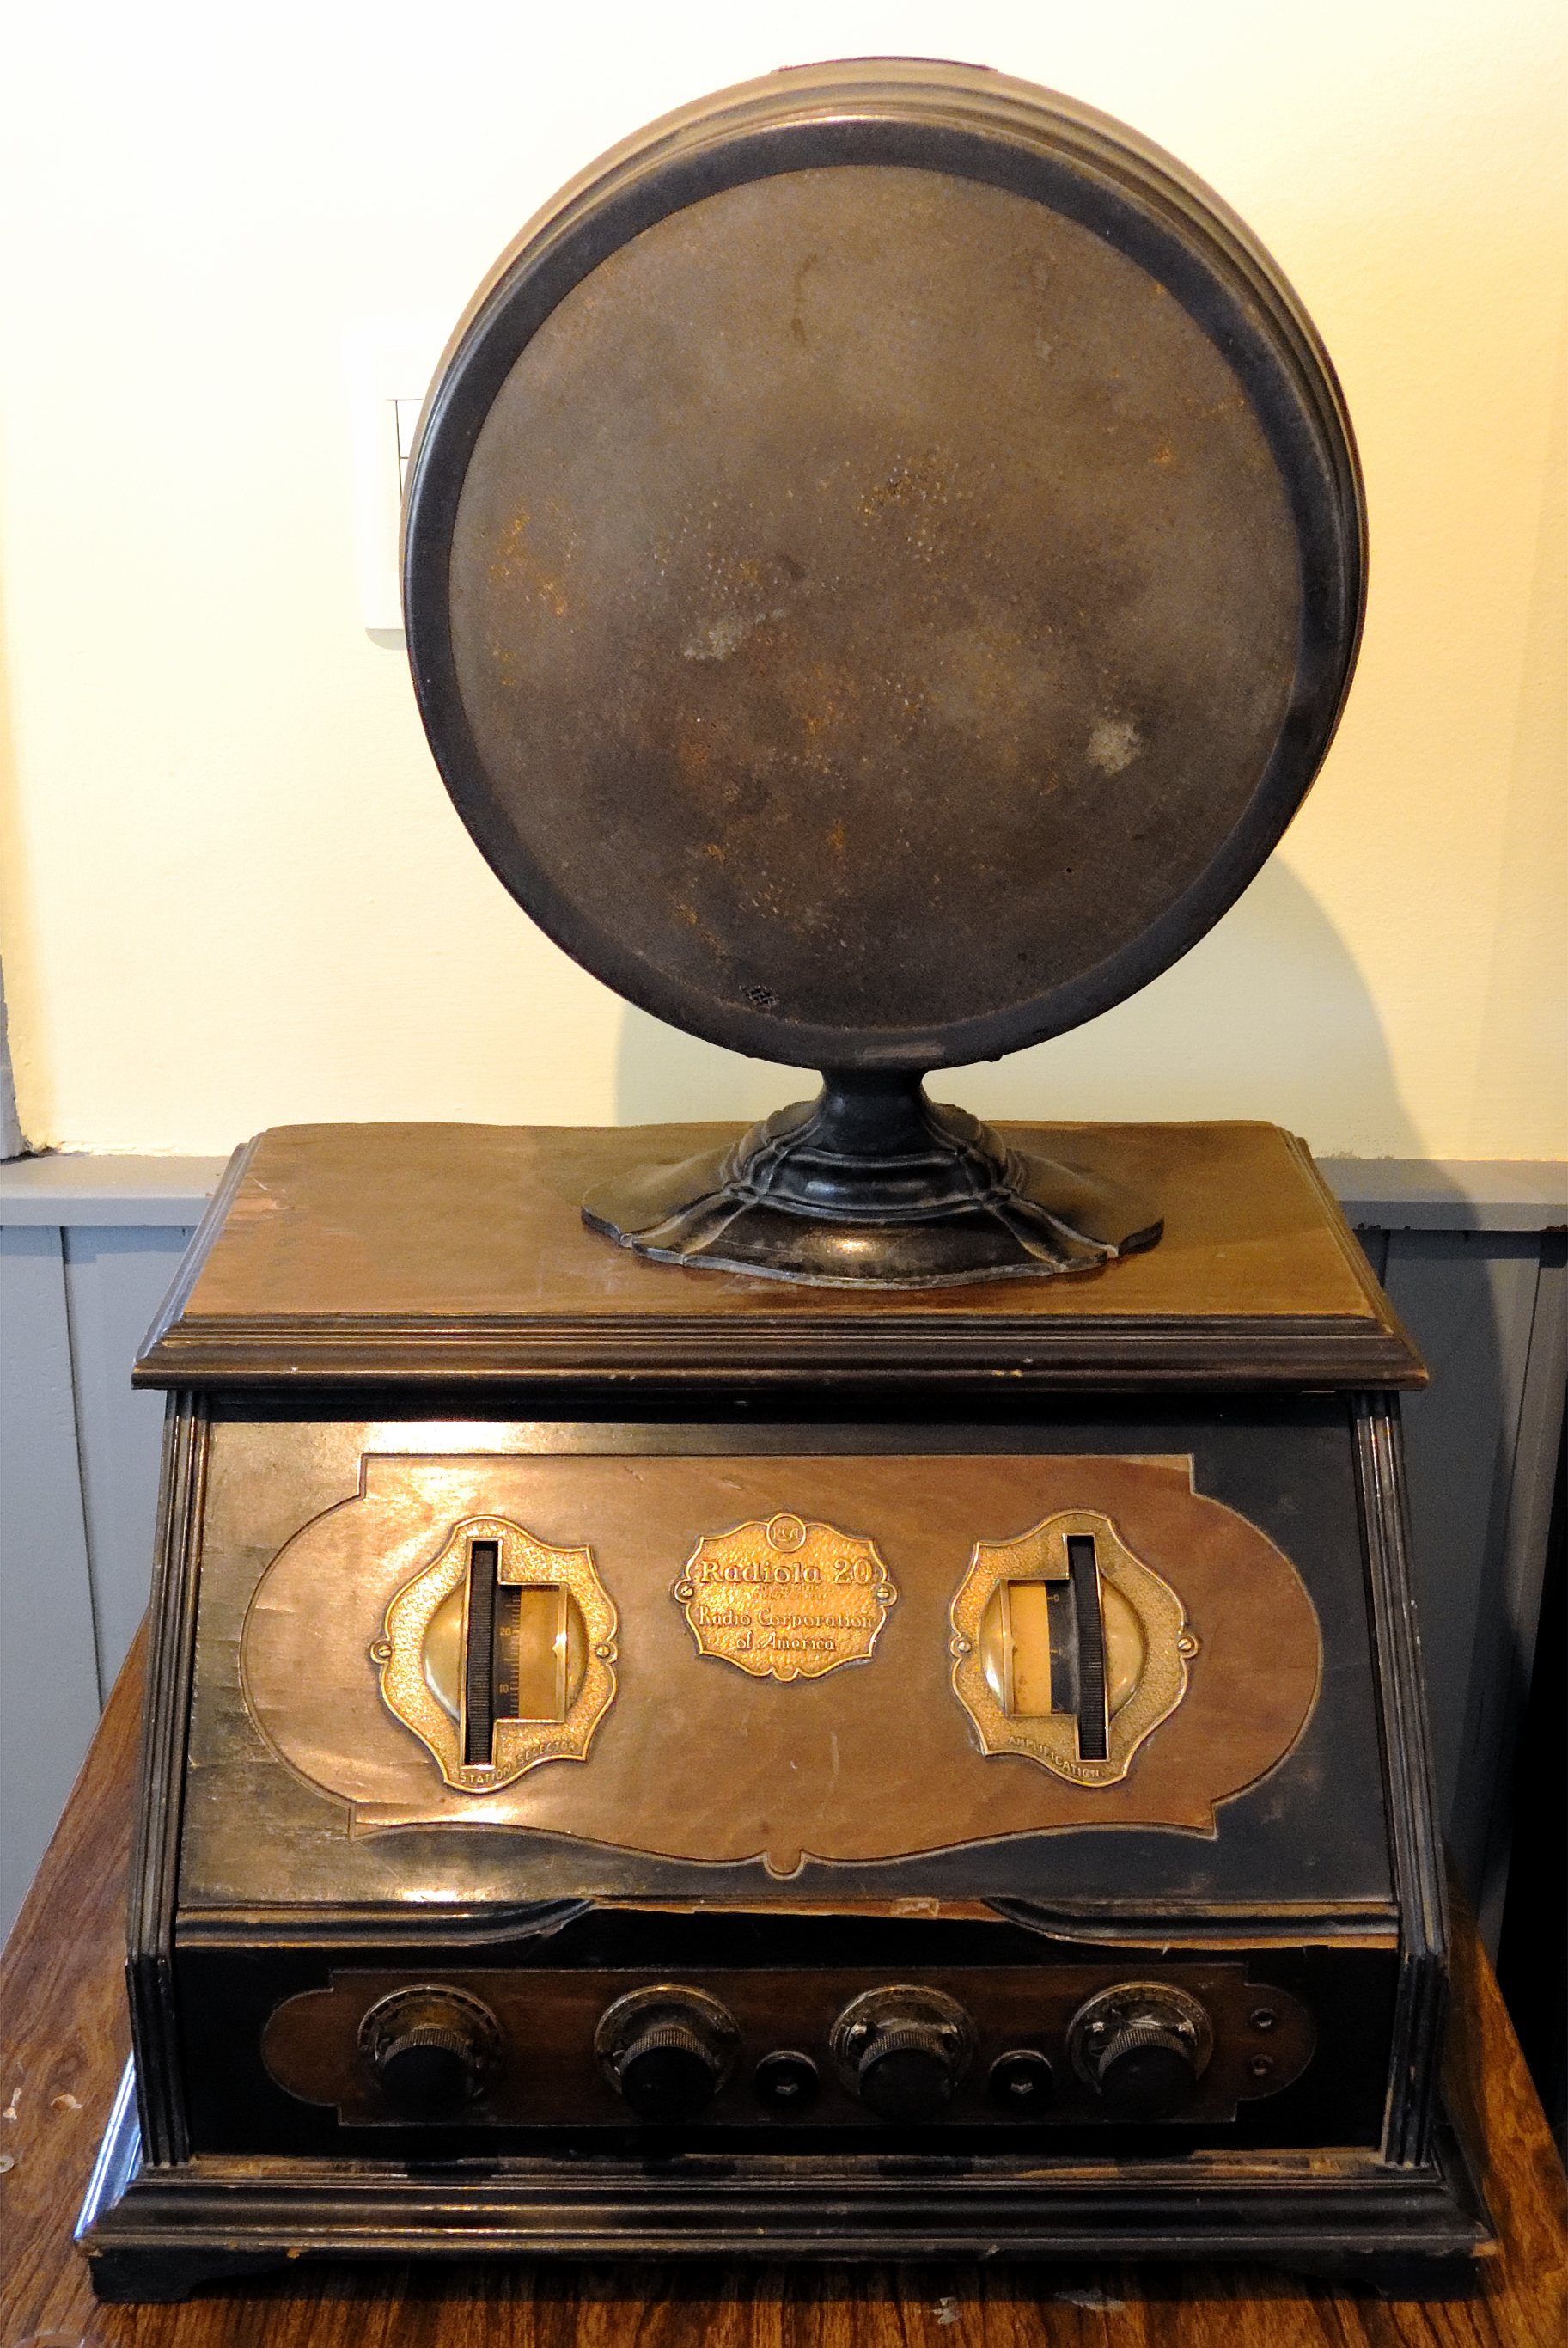
\includegraphics[width=0.55\textwidth]{../figures/early_radio.jpg}
        \caption{Radio primitiva. \cite{wiki:historia_radio}}
      \end{figure}
    \end{column}
  \end{columns}
\end{frame}

\begin{frame}{Aislamiento en Tubos de Vacío}
  \frametitle{Componentes Críticos para Válvulas Termoiónicas}
  Los \textbf{tubos de vacío} fueron el componente activo central de la
  electrónica en la primera mitad del siglo XX.

  \begin{columns}[T]
    \begin{column}{0.6\textwidth}
      \begin{itemize}[<+->]
        \item Las bases de estos dispositivos debían ser excelentes aislantes y
          soportar el calor de operación.
        \item Se fabricaron con \textbf{porcelana} y \textbf{esteatita},
          asegurando el aislamiento y la integridad estructural.
      \end{itemize}
    \end{column}
    \begin{column}{0.4\textwidth}
      \begin{figure}
        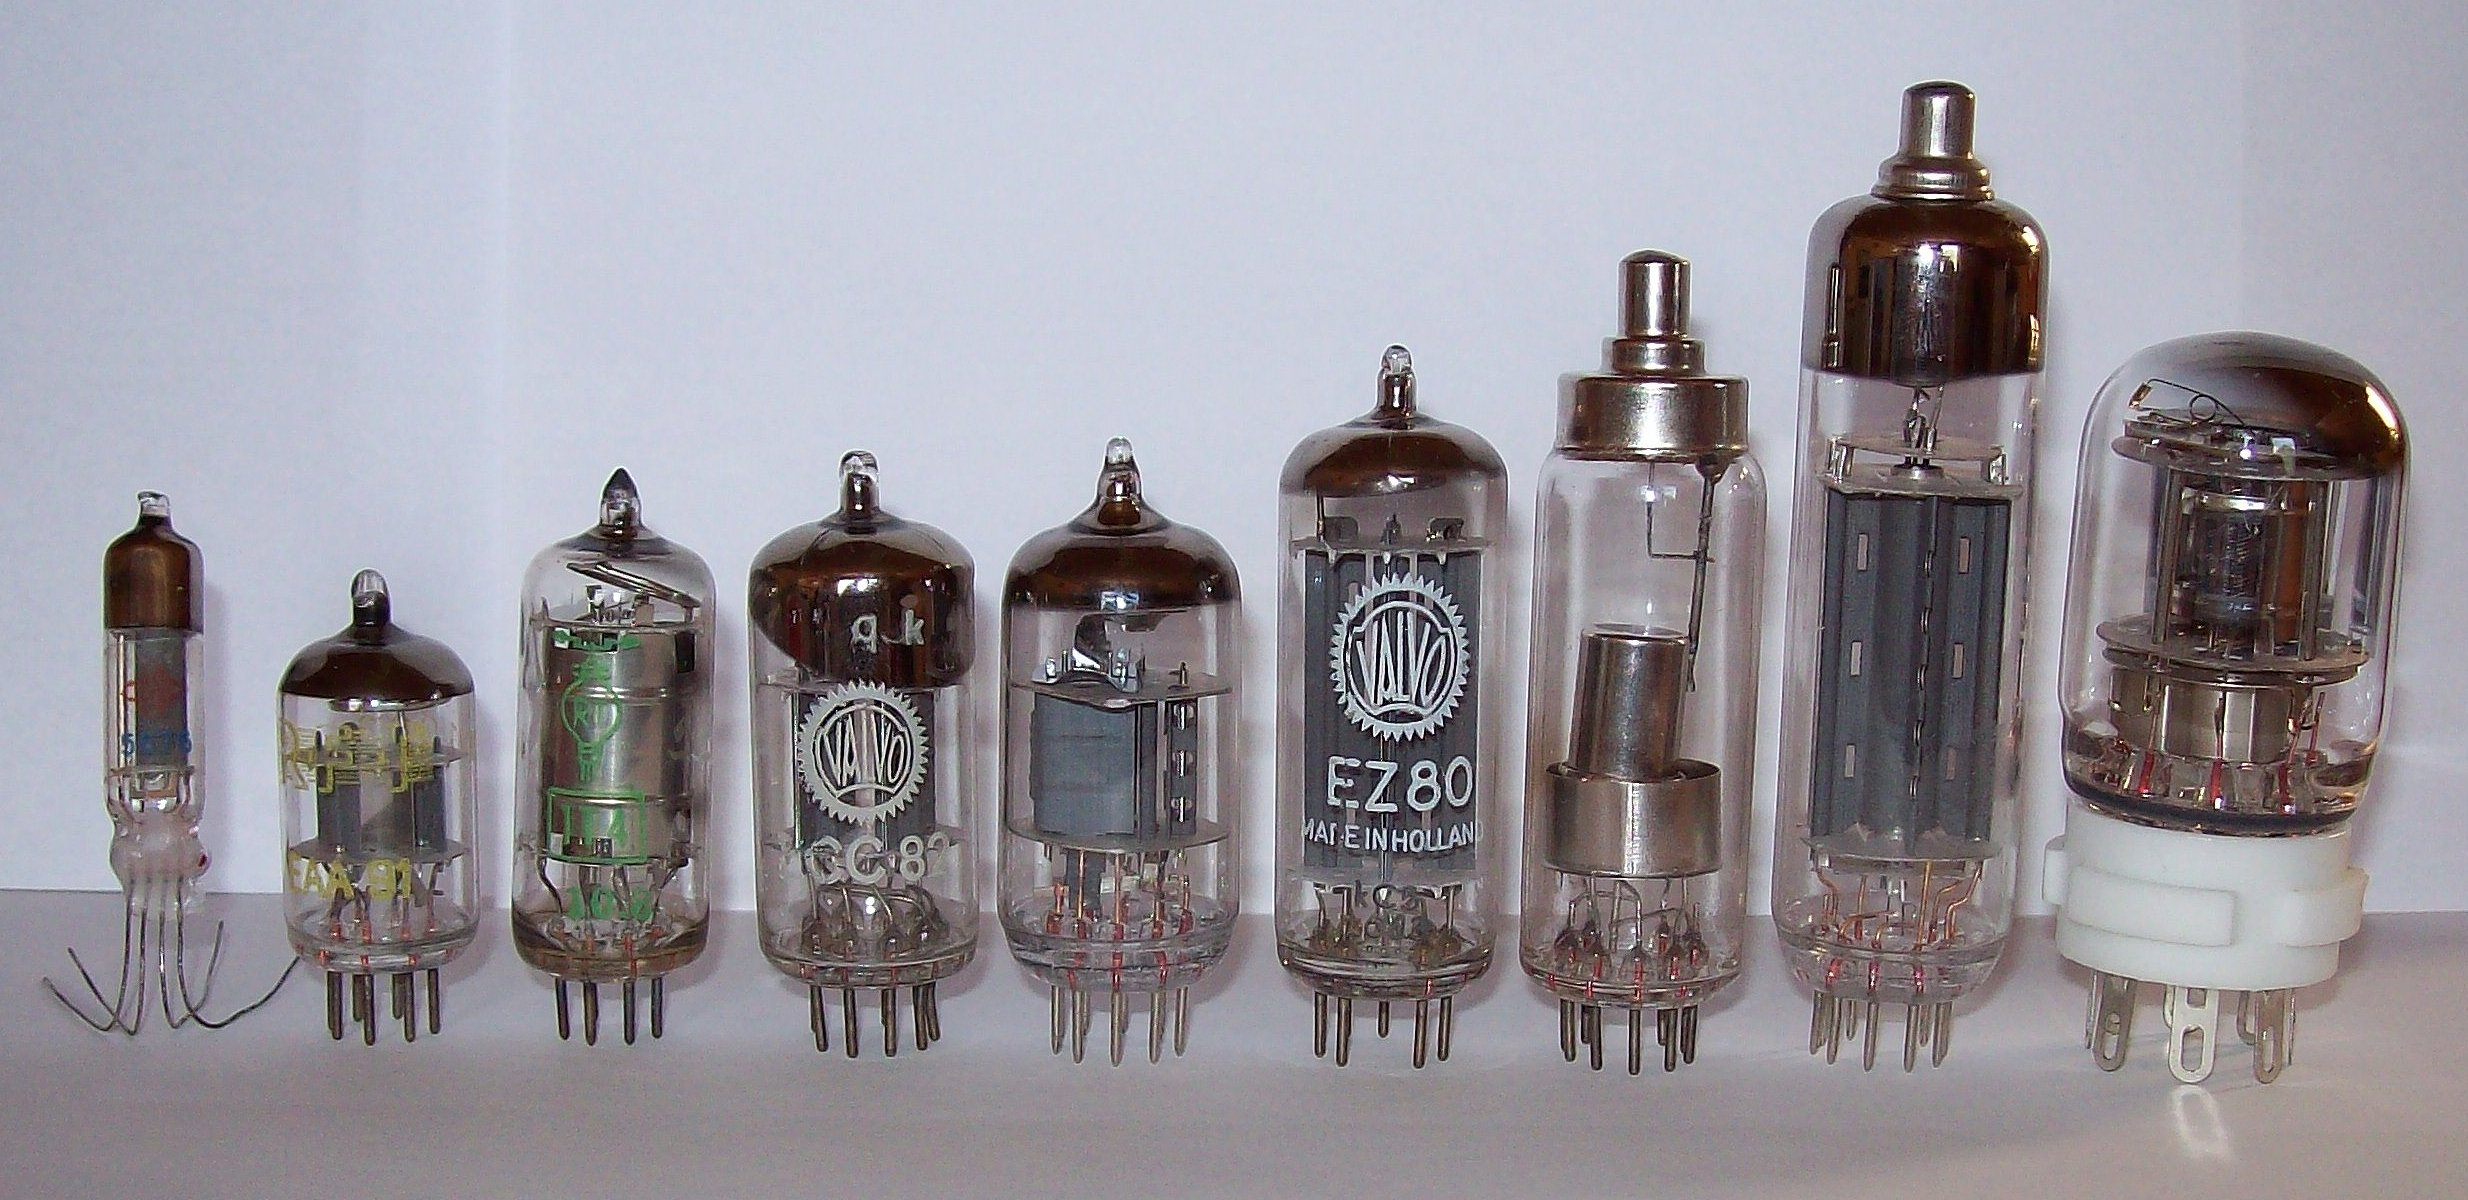
\includegraphics[width=\textwidth]{../figures/vacuum_tubes.jpg}
        \caption{Tubos de vacío. \cite{wiki:vacuum_tube}}
      \end{figure}
    \end{column}
  \end{columns}
\end{frame}

\begin{frame}{Sustratos para Componentes Pasivos}
  \frametitle{Soportes Dieléctricos para Circuitos}
  La construcción de circuitos requería componentes pasivos como resistencias y
  capacitores.

  \begin{columns}[T]
    \begin{column}{0.6\textwidth}
      \begin{itemize}[<+->]
        \item Se utilizaron cerámicos como el \textbf{cuerpo o sustrato
          aislante} de dichos componentes.
        \item El material cerámico proveía el soporte mecánico, el aislamiento
          eléctrico y la disipación de calor.
      \end{itemize}
    \end{column}
    \begin{column}{0.4\textwidth}
      \begin{figure}
        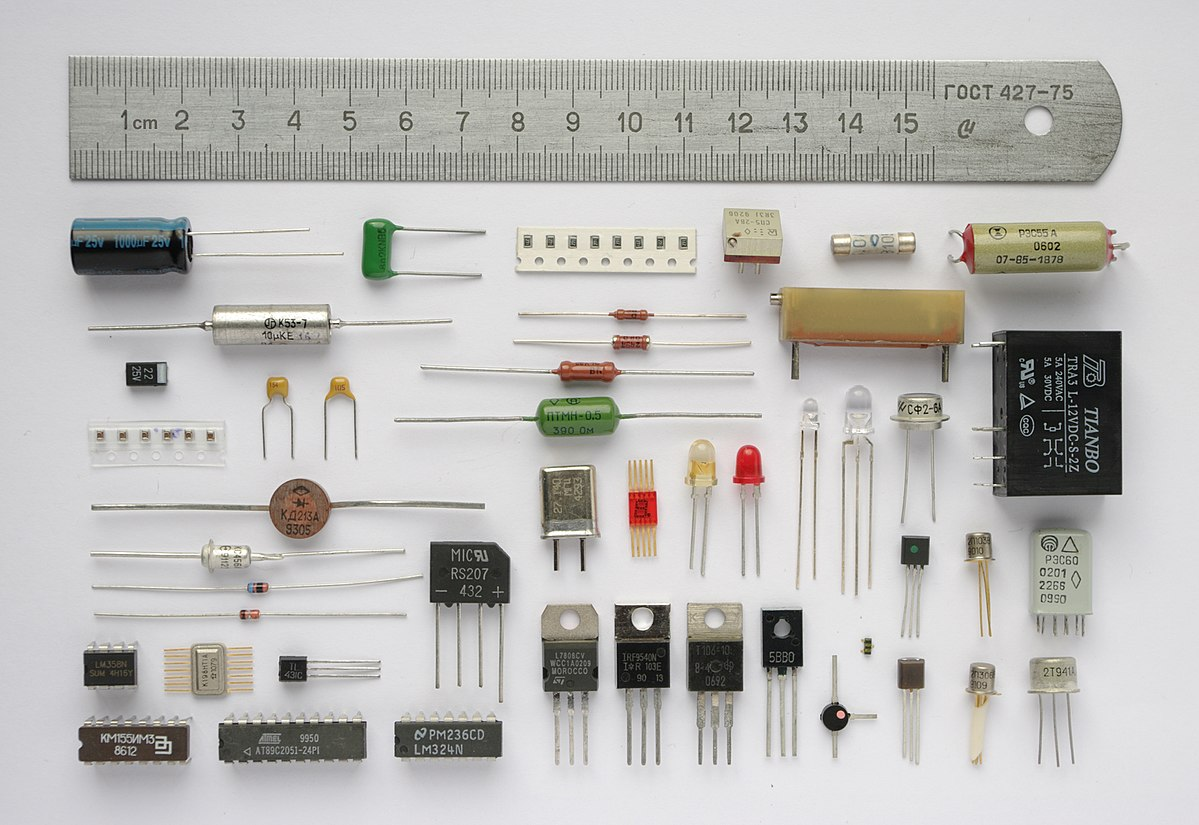
\includegraphics[width=\textwidth]{../figures/passive_components.jpg}
        \caption{Componentes electricos. \cite{wiki:electronic_component}}
      \end{figure}
    \end{column}
  \end{columns}
\end{frame}

\begin{frame}{Puntos importantes}
  \frametitle{Conclusiones}
  \begin{itemize}[<+->]
    \item En el período analizado (1750-1950), la cerámica se consolidó como un
      \textbf{material de ingeniería} indispensable.
    \item Si bien no fue una tecnología principal, funcionó como una
      \textbf{tecnología habilitadora fundamental}.
    \item Sus propiedades refractarias, de inercia química y de aislamiento
      dieléctrico fueron un requisito previo para el desarrollo de la
      siderurgia, la industria química y la electrificación.
  \end{itemize}
\end{frame}


\section{Aplicaciones Modernas}

\begin{frame}{Primeros Desarrollos y Aplicaciones (1950 - 1970)}
  El periodo de posguerra requirió materiales con un rendimiento superior al de
  los metales en condiciones específicas.

  \begin{block}{Material: Alúmina (\ce{Al2O3})}
    \begin{itemize}[<+->]
      \item \textbf{Propiedad Clave:} Alto aislamiento dieléctrico y
        resistencia térmica.
      \item \textbf{Aplicación:} Aisladores de bujías en motores y sustratos
        para circuitos electrónicos.
    \end{itemize}
  \end{block}

  \begin{block}{Material: Circonia (\ce{ZrO2})}
    \begin{itemize}[<+->]
      \item \textbf{Propiedad Clave:} Muy baja conductividad térmica y alta
        estabilidad.
      \item \textbf{Aplicación:} Recubrimientos de barrera térmica (TBC) en
        componentes de motores a reacción.
    \end{itemize}
  \end{block}
\end{frame}

\begin{frame}{Aplicaciones en Electrónica y Biomedicina (1980 - 2000)}
  \begin{block}{Componentes Electrónicos y Sensores}
    \begin{itemize}[<+->]
      \item \textbf{Materiales:} Titanato de Bario (\ce{BaTiO3}),
        Titanato-zirconato de plomo (PZT).
      \item \textbf{Propiedades Clave:} Alta constante dieléctrica y efecto
        piezoeléctrico.
      \item \textbf{Aplicaciones:} Condensadores cerámicos multicapa (MLCC),
        transductores para ultrasonido.
    \end{itemize}
  \end{block}

  \begin{block}{Biomateriales}
    \begin{itemize}[<+->]
      \item \textbf{Materiales:} Circonia y Alúmina de grado médico.
      \item \textbf{Propiedades Clave:} Biocompatibilidad y alta resistencia al
        desgaste.
      \item \textbf{Aplicaciones:} Implantes dentales y componentes de prótesis
        articulares (ej. cabezas femorales).
    \end{itemize}
  \end{block}
\end{frame}


\begin{frame}{Materiales para Sectores de Alto Rendimiento (2000 - Hoy)}
  La mejora en la tenacidad y fiabilidad ha permitido su uso en aplicaciones
  estructurales críticas.

  \begin{itemize}[<+->]
    \item \textbf{Aeroespacial:} Compuestos de Matriz Cerámica (CMC, ej. \ce{SiC/SiC})
      para componentes de motores a reacción, permitiendo mayor eficiencia de
      combustión.
      \vspace{0.5cm}
    \item \textbf{Blindaje y Protección:} Carburo de silicio (\ce{SiC}) y carburo
      de boro (\ce{B4C}) para blindaje personal y de vehículos por su extrema
      dureza y baja densidad.
      \vspace{0.5cm}
    \item \textbf{Generación de Energía:} Circonia estabilizada con itria (YSZ)
      como electrolito en celdas de combustible de óxido sólido (SOFC) por su
      conductividad iónica.
  \end{itemize}
\end{frame}

\begin{frame}{Cerámicas Superconductoras de Alta Temperatura (HTS)}
  Un descubrimiento disruptivo en la física de materiales fue la
  superconductividad en compuestos cerámicos.

  \pause

  \begin{block}{Descubrimiento Clave (1986)}
    Bednorz y Müller descubrieron superconductividad en un óxido cerámico de la
    familia de los cupratos a una temperatura superior a la de cualquier
    superconductor metálico conocido. Este hito les valió el \alert{Premio
    Nobel} de
    Física en 1987.
  \end{block}

  \pause

  \begin{block}{Material Principal y Propiedades}
    \begin{itemize}[<+->]
      \item \textbf{Ejemplo:} Óxido de Itrio, Bario y Cobre (YBCO), con fórmula
        \ce{YBa2Cu3O_{7-\delta}}.
      \item \textbf{Estructura:} Cristalina compleja de tipo perovskita.
      \item \textbf{Desafío Técnico:} Su naturaleza cerámica les confiere una
        alta fragilidad, dificultando su fabricación en forma de cables
        flexibles.
    \end{itemize}
  \end{block}
\end{frame}

\begin{frame}
  \begin{block}{Impacto y Aplicaciones}
    La capacidad de ser superconductores a temperaturas superiores a la del
    nitrógeno líquido (77 K, -196 °C) redujo drásticamente los costes de
    enfriamiento. Sus aplicaciones incluyen:
    \begin{itemize}[<+->]
        \item Imanes de alto campo para resonancia magnética (RM) y
          aceleradores de partículas.
        \item Limitadores de corriente de falla en redes eléctricas.
        \item Transporte por levitación magnética (Maglev).
     \end{itemize}
  \end{block}
\end{frame}

\begin{frame}{Fronteras Actuales: Computación Cuántica y Óptica Avanzada}
  \begin{block}{Computación Cuántica}
    \begin{itemize}[<+->]
      \item \textbf{Materiales:} Sustratos monocristalinos de Zafiro (\ce{Al2O3})
        y Nitruro de Silicio (\ce{Si3N4}).
      \item \textbf{Función:} Sus bajas pérdidas dieléctricas a temperaturas
        criogénicas son esenciales para fabricar resonadores que interactúan
        con cúbits superconductores, minimizando la decoherencia.
    \end{itemize}
  \end{block}

  \begin{block}{Cerámicas Transparentes}
    \begin{itemize}[<+->]
      \item \textbf{Materiales:} Oxinitruro de Aluminio (ALON), Espinela
        (\ce{MgAl2O4}).
      \item \textbf{Aplicación:} Ventanas para sensores militares y blindaje
        transparente, combinando dureza con transparencia óptica.
    \end{itemize}
  \end{block}
\end{frame}


\section{Referencia}
\begin{frame}[allowframebreaks]{References}
	\printbibliography
	\nocite{*}
\end{frame}

\begin{frame}[plain]
	\centering
	\vspace{1cm}
	{\Huge \textbf{Gracias!}}\\[1cm]
	{\large Preguntas o comentarios?}
\end{frame}

\end{document}
